\begin{figure}[t]
  \centering
  \resizebox{\columnwidth}{!}{%
  \begin{tikzpicture}[
      font=\small,
      screenshot/.style={
        rectangle,
        draw=black!65,
        inner sep=0pt
      },
      decision/.style={
        diamond,
        aspect=1.6,
        draw=black!65,
        fill=yellow!12,
        minimum width=20mm,
        minimum height=12mm,
        align=center,
        font=\small\bfseries
      },
      result/.style={
        rectangle,
        rounded corners=2pt,
        draw=black!65,
        minimum width=27mm,
        minimum height=11mm,
        align=center,
        font=\small\bfseries
      },
      arrow/.style={-{Latex[length=2.2mm]}, thick, draw=black!70},
      pics/check icon/.style={code={
        \draw[green!55!black, line width=2.2pt, line cap=round,
          line join=round] (-.32,.00) -- (-.09,-.23) -- (.38,.28);
      }}
    ]

    \node[screenshot] (initial) at (0,1.9) {
      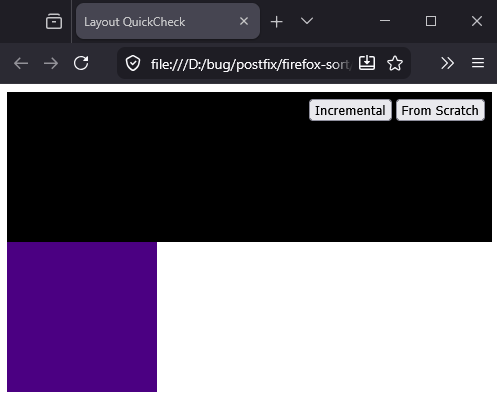
\includegraphics[width=42mm]{figures/init-page.png}
    };
    \node[screenshot] (incremental) at (5.7,1.9) {
      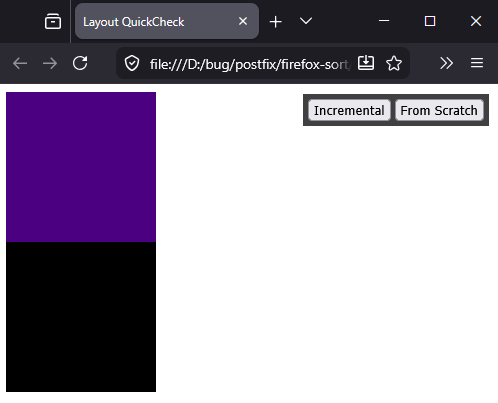
\includegraphics[width=42mm]{figures/inc-page.png}
    };
    \node[screenshot] (scratch) at (5.7,-2.5) {
      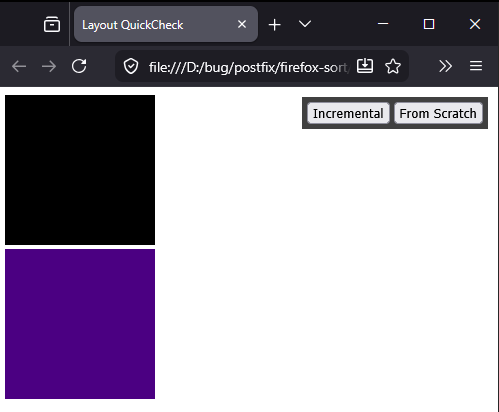
\includegraphics[width=42mm]{figures/fresh-page.png}
    };

    \node[
      font=\small\bfseries,
      anchor=south,
      fill=white,
      fill opacity=.8,
      text opacity=1,
      inner sep=1pt
    ] at ([yshift=2.5mm]initial.south) {Initial page};
    \node[
      font=\small\bfseries,
      anchor=south,
      fill=white,
      fill opacity=.8,
      text opacity=1,
      inner sep=1pt
    ] at ([yshift=2.5mm]incremental.south) {Incremental Layout};
    \node[
      font=\small\bfseries,
      anchor=south,
      fill=white,
      fill opacity=.8,
      text opacity=1,
      inner sep=1pt
    ] at ([yshift=2.5mm]scratch.south) {From-Scratch Layout};

    \node[
      decision,
      draw=red!65!black,
      fill=red!12
    ] (equal) at (9.8,-.15)
      {Layouts\\equal?\\\textcolor{red!65!black}{No}};
    \node[result, fill=green!14] (no-bug) at (13.2,1.2)
      {\hspace{7mm}No bug};
    \node[result, fill=red!14] (bug) at (13.2,-1.5)
      {\hspace{7mm}Bug};

    \pic[scale=.72] at ([xshift=-8mm]no-bug.center) {check icon};
    \node at ([xshift=-8mm]bug.center) {
      
\includegraphics[width=6mm]{figures/bug.png}
    };

    \draw[arrow] (initial) --
      node[above, font=\scriptsize\bfseries, align=center] {Apply\\Changes}
      (incremental);
    \draw[arrow] (incremental) --
      node[right, font=\scriptsize\bfseries, align=left]
        {Recompute\\from Scratch}
      (scratch);
    \draw[arrow] (incremental) -- (equal);
    \draw[arrow] (scratch) -- (equal);
    \draw[-{Latex[length=2.2mm]}, draw=black!35, dashed] (equal) --
      node[above, font=\scriptsize, text=black!45] {Yes}
      (no-bug);
    \draw[-{Latex[length=2.2mm]}, very thick, draw=red!65!black] (equal) --
      node[below, font=\scriptsize\bfseries, text=red!65!black] {No}
      (bug);
  \end{tikzpicture}
  }
  \caption{Example execution of the self-differential oracle. Starting from
    the initial page, \toolname applies changes incrementally and recomputes
    the changed page from scratch. Different resulting layouts indicate an
    under-invalidation bug.}
  \label{fig:oracle-example}
\end{figure}
